\documentclass[a4paper]{scrartcl}

\usepackage[
fancytheorems, 
fancyproofs, 
noindent, 
%  spacingfix,  
]{adam}

\usepackage{tikz}
\usetikzlibrary{automata, positioning}

\title{Markov Chains}
\author{Adam Kelly (\texttt{ak2316@cam.ac.uk})}
\date{\today}


\allowdisplaybreaks

\begin{document}

\maketitle

A stochastic process is said to have the `Markov property' if, conditional on its present value, the future is independent of the past.
This is a \emph{restrictive} assumption, but we do end up with a useful model with a rich mathematical theory, which we shall study in this course.

This article constitutes my notes for the `Markov Chains' course, held in Michaelmas 2021 at Cambridge. These notes are \emph{not a transcription of the lectures}, and differ significantly in quite a few areas. Still, all lectured material should be covered.


\tableofcontents

% \clearpage

\section{The Markov Property}

\subsection{What is a Markov Chain?}

Let $S$ be a countable set (the set of possible `states'), and let $X_n$ be a sequence of random variables taking values in $S$.

\begin{definition}[Markov Chain]
	The sequence of random variables $X_n$ is a \vocab{Markov chain} if it satisfies the \vocab{Markov property}
	$$
	\PP(X_{n + 1} = x_{n + 1} \mid X_n = x_n, X_0 = x_0) = \PP(X_{n + 1} = x_{n + 1} \mid X_n = x_n).
	$$

	The Markov chain is said to be \vocab{homogeneous} if for all $i, j \in S$ the conditional probability $\PP(X_{n + 1} = j \mid X_n = i)$ is independent of $n$.
\end{definition}

In this course we are only going to study homogeneous Markov chains.

Markov chains are often best described by diagrams\footnote{You might notice that these diagrams are labelled directed graphs, and indeed you will see concepts from graph theory such as connectivity reoccur when we later talk about communicating classes.} which show the probability of moving from one state to another.
For example, the Markov chain in the diagram below has three states which we label $\{1, 2, 3\}$, and the probability of moving from state 1 to state 2 is $1/2$, and the probability of moving from state 2 to state 3 is $1/3$, and so on.

\begin{center}
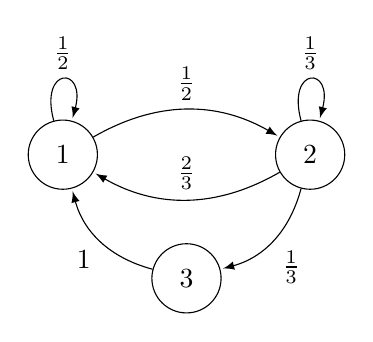
\begin{tikzpicture}

\node[state] (1) {1};
\node [right=of 1] (4) {};
\node[state, right=of 4] (2) {2};
\node[state, below=of 4] (3) {3};

\draw[every loop, >=latex]
(1) edge[loop above] node {$\frac{1}{2}$} (1)
(1) edge[bend left, auto=left] node {$\frac{1}{2}$} (2)
(2) edge[bend left, auto=left] node[above] {$\frac{2}{3}$} (1)
(2) edge[loop above] node {$\frac{1}{3}$} (2)
(2) edge[bend left, auto=left] node {$\frac{1}{3}$} (3)
(3) edge[bend left, auto=left] node {$1$} (1);

\end{tikzpicture}
\end{center}

In general, to calculate the probabilities associated with a Markov chain, we need to know two quantities.

\begin{itemize}
	\item \emph{The initial distribution}. We first need to know about the starting state of a Markov chain. This is described by the initial distribution $\lambda = (\lambda_i \mid i \in S)$, where $\lambda_i = \PP(X_0 = i)$.
	\item \emph{The transition probabilities}. We also need to know the probability of moving from a state $i \in S$ to a state $j \in S$. This is typically given by a \emph{transition matrix} $P = (P_{i, j} \mid i, j \in S)$ with $p_{i,j} = \PP(X_1 = j \mid X_0 = i)$.
\end{itemize}
These quantities are of course subject to some constraints, in that we require $\sum_{i \in S} \lambda_i = 1$ and the transition matrix $P$ must be \vocab{stochastic}, in that $\sum_{j \in S} P_{i, j} = 1$ for all $i \in S$.

If a Markov chain $X_n$ has initial distribution $\lambda$ and transition matrix $P$, we say that it is \vocab{$\markov(\lambda, P)$}.

Once we have these quantities, we can begin to actually establish various properties about the Markov chain, for example the probability that it goes through a given sequence of states.

\begin{theorem}[Probability of a Sequence of States]
	The sequence of random variables $X_n$ is $\markov(\lambda, P)$ if and only if
	$$
	\PP(X_0 = i_0, X_1 = i_1, \dots, X_n = i_n) = \lambda_{i_0}P_{i_0, i_1} \cdots P_{i_{n - 1}, i_n},
	$$
	for all $n \geq 0$ and $i_0, \dots, i_n \in S$.
\end{theorem}
\begin{proof}
	Let $A_k$ denote the event $\{X_k = i_k\}$. First suppose that $X_n$ is $\markov(\lambda, P)$. We prove the result holds by induction. For $n = 0$ this is true by definition. Then if it holds up to $n$, we have
	\begin{align*}
	\PP(A_0 \cap \cdots \cap A_n)  &= \PP(A_0 \cap \cdots \cap A_{n - 1})\PP(A_n \mid A_0 \cap \cdots \cap A_{n - 1}) \\
	&= \PP(A_0 \cap \cdots \cap A_{n - 1})\PP(A_n \mid A_{n - 1}) \\ 
	&= \left(\lambda_{i_0}P_{i_0, i_1} \cdots P_{i_{n - 2}, i_{n - 1}}\right)P_{i_{n - 1}, i_n},
\end{align*}
which completes our induction.

Conversely, suppose that the result holds. Then with $n = 0$ we get that the initial distribution of $X_n$ is $\lambda$. Then
$$
\PP(A_{n + 1} \mid A_{0} \cap \cdots \cap A_n) = \frac{\PP(A_0 \cap \cdots \cap A_{n + 1})}{\PP(A_0 \cap \cdots \cap A_{n})} = P_{i_{n}, i_{n + 1}}.
$$
Since this does not depend on $i_0, \dots, i_{n - 1}$, $X_n$ is a homogeneous Markov chain with transition matrix $P$, as required.
\end{proof}

\subsection{Simple Markov Property}

An important aspect of Markov chains is that they are \emph{memoryless}, in the future is independent of the past, conditional on the present. This is encapsulated in the \vocab{simple Markov property}.

\begin{theorem}[Simple Markov Property]
	Let $X_n$ be a Markov chain. Then conditional on $X_m = i$, the sequence of random variables $(X_{m + n})_{n \geq 0}$ is\footnote{Here $\delta_{ij}$ is 1 if $i = j$ and 0 otherwise.} $\markov(\delta_i, P)$, and is independent of $X_0, \dots, X_m$.
\end{theorem}
\begin{proof}
	Given any event $H$ determined by $X_0, \dots, X_m$, we want to show that for an event $F = \{X_m = i_m, \dots X_{m + n} = i_{m +n}\}$ we have
	$$
	\PP(H \cap F \mid X_m = i) = \delta_{ii_m}P_{i_m, i_{m + 1}} \cdots P_{i_{m + n-1}, i_{m + n}} \PP(H \mid X_m = i).
	$$
	Indeed, considering the case of $H = \{X_0 = i_0, \dots, X_m = i_m\}$ we have
	\begin{align*}
		\PP(H \cap F \mid X_m = i) &= \frac{\lambda_{i_0}P_{i_0, i_1} \cdots P_{i_{m - 1}, i}P_{i, i_{m + 1}} \cdots P_{i_{m + n - 1}, i_{m + n}}}{\PP(X_m = i)} \\
		&= \delta_{i i_m}P_{i, i_{m + 1}} \cdots P_{i_{m + n - 1}, i_{m + n}} \PP(H \mid X_m = i),
	\end{align*}
	as required. 
	
	Then for a general $H$, we can write it as the disjoint union $H = \bigcup_{k = 1}^{\infty} H_k$, and then the overall result follows by summing the above result for relevant $H_k$.
\end{proof}

\subsection{Transition Probabilities}

We are now going to address how to find the probability that a Markov chain is in a given state after $n$ steps.
The core idea of this section is that we will be able to reduce such questions into questions about the transition matrix that we introduced earlier.

Recall that if $X_n$ is a Markov chain with transition matrix $P$, then $P_{i, j}$ was the probability of moving from the state $i$ to the state $j$. We call these the \vocab{one-step transition probabilities}. We can generalize this slightly.

\begin{definition}[$n$-Step Transition Probabilities]
	For a Markov chain $X_n$, the \vocab{$n$-step transition probabilities} are given by
	$$
	p_{i, j}(n) = \PP(X_n = j \mid X_0 = i).
	$$
\end{definition}

These $n$-step transition probabilities naturally form the \vocab{$n$-step transition matrix} $P(n) = (p_{i, j}(n) \mid i, j \in S)$. The nice thing about writing these transition probabilities as a matrix is that they satisfy a lovely set of equations that relate extremely well to matrix algebra.

\begin{theorem}[Chapman-Kolmogorov Equations]
	We have that
	$$
	p_{i, j}(n + m) = \sum_{k \in S} p_{i, k}(n)p_{k, j}(m),
	$$
	where $i, j \in S$ and $m, n \geq 0$. In particular, $P(m + n) = P(m)P(n)$.
\end{theorem}
\begin{proof}
	Using the partition theorem and simple Markov property,
	\begin{align*}
		p_{i, j}(n + m) &= \PP(X_{n + m} = j \mid X_0 = i) \\
		&= \sum_{k \in S} \PP(X_{m + n} = j \mid X_n = k, X_0 = i) \PP(X_n = k \mid X_0 = i) \\
		&= \sum_{k \in S} \PP(X_{m + n} = j \mid X_n = k) \PP(X_n = k \mid X_0 = i) \\
		&= \sum_{k \in S} p_{i, k}(n) p_{k, j}(m).
	\end{align*}
\end{proof}

So, if we have some $n$-step transition matrix $P(n)$, the above result shows us that it satisfies $P(n) = P^n$. This reduces our problem to just this:

\begin{center}
	\color{blue}
	To compute $p_{i, j}(n)$, we can compute powers of\\ the transition matrix, and take $(P^n)_{i, j}$.
\end{center}

In general, this makes our problem significantly easier, and if the state space is finite, we can use tools from linear algebra such as diagonalisation.

\begin{example}[Computing Transition Probabilities]
	Let $\alpha, \beta \in (0, 1)$. 
	Consider the Markov chain $X_n$ with states $S = \{1, 2\}$, with transition matrix 
	$$
	P = \begin{pmatrix}
		1 - \alpha & \alpha \\
		\beta & 1 - \beta
	\end{pmatrix}.
	$$
	A diagram of this markov chain is shown below.
	\begin{center}
	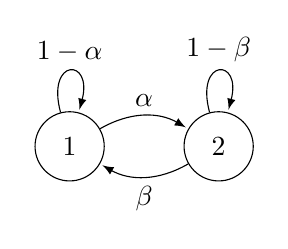
\begin{tikzpicture}

	\node[state] (1) {1};
	\node[state, right=of 1] (2) {2};

	\draw[every loop, >=latex]
	(1) edge[loop above] node {$1 - \alpha$} (1)
	(1) edge[bend left, auto=left] node {$\alpha$} (2)
	(2) edge[bend left, auto=left] node {$\beta$} (1)
	(2) edge[loop above] node {$1 -\beta$} (2);

	\end{tikzpicture}
	\end{center}

	We want to find the $n$-step transition probabilities.

	\textbf{Method 1} (Difference Equations). We are first going to find $p_{1, 1}(n)$ using a `bare-hands' method. By the Chapman-Kolmogorov equations (that is, conditioning on $X_n$) we have
	\begin{align*}
		p_{1, 1}(n + 1) &= p_{1, 1}(n)p_{1, 1}(1) + p_{1, 2}(n) p_{2, 1}(1) \\
		&= (1 - \alpha)p_{1, 1}(n) + \beta p_{1, 2}(n) \\
		&= (1 - \alpha)p_{1, 1}(n) + \beta (1 - p_{1, 1}(n)) \\
		&= p_{1, 1}(n)(1 - \alpha - \beta) + \beta.
	\end{align*}
	This is a recurrence relation which we can then solve using the boundary condition $p_{1, 1}(0) = 1$ to get
	$$
		p_{1, 1}(n) = \begin{cases}
			\frac{\alpha}{\alpha+\beta}+\frac{\alpha}{\alpha+\beta} \cdot(1-\alpha-\beta)^{n} &\mbox{if } \alpha + \beta > 0, \\
			1 &\mbox{if } \alpha + \beta = 0.
		   \end{cases}
	$$

	\textbf{Method 2} (Diagonalisation). An alternative solution uses some tools from matrix algebra. To calculate the $n$-step transition matrix $P^n$, we are going to diagonalise $P$.

	The eigenvalues of $P$ are given by the solutions to $\det(P - \mu I) = 0$, which are $\{1, 1 - \alpha - \beta\}$. Thus for some invertible matrix $U$ we have
	$$
	P = U^{-1}\begin{pmatrix}
		1 & 0 \\ 0 & 1 - \alpha - \beta
	\end{pmatrix}U \quad \text{and} \quad P^n = U^{-1} \begin{pmatrix}
		1 & 0 \\ 0 & (1 - \alpha - \beta)^n
	\end{pmatrix}U.
	$$
	Thus $p_{1, 1}(n) = A + B(1 - \alpha - \beta)^n$, for constants $A$ and $B$. We can find these by noting the boundary conditions $p_{1, 1}(0) = 1$ and $p_{1, 1}(1) = 1 - \alpha$, giving 
	$$
		p_{1, 1}(n) = \begin{cases}
			\frac{\alpha}{\alpha+\beta}+\frac{\alpha}{\alpha+\beta} \cdot(1-\alpha-\beta)^{n} &\mbox{if } \alpha + \beta > 0, \\
			1 &\mbox{if } \alpha + \beta = 0.
		   \end{cases}
	$$
\end{example}

In general, if the state space of a Markov chain is finite with $|S| = k$, then $P$ is a $k \times k$ matrix with eigenvalues $\mu_1, \dots, \mu_k$.

If \emph{all of the eigenvalues are distinct}, then $P$ is diagonalisable, and we can write
$$
P = U^{-1} \begin{pmatrix}
	\mu_1 & \cdots & 0 \\
	0 & \ddots & 0 \\
	0 & \cdots & \mu_k
\end{pmatrix} U \quad \text{and} \quad P^n = U^{-1} \begin{pmatrix}
	\mu_1^n & \cdots & 0 \\
	0 & \ddots & 0 \\
	0 & \cdots & \mu_k^n
\end{pmatrix} U,
$$
and $p_{i,j} = a_1 \mu_1^n + \cdots + a_k \mu_k^n$, for some constants $a_1, \dots, a_k$, which are determined by the boundary conditions.

If some eigenvalue $\mu_k$ is complex, then it's conjugate is also an eigenvalue, so if $\mu_k = re^{i \theta}$ we have also the eigenvalue $\overline{\mu_k} = re^{-i \theta}$, and we can write
$$
p_{i, j} = a_1 \mu_1^n + \cdots + a_{k - 2}\mu_{k - 2}^n + a_{k - 1}r^n \cos(n \theta) + a_k r^n \sin (n \theta),
$$
since $p_{i, j}$ is real and so all of the imaginary parts must cancel out.


If \emph{some eigenvalues repeat}, then the situation is slightly more complicated. If an eigenvalue $\mu_k$ has multiplicity $m$, we can simply replace $a_k$ by a degree $m$ polynomial in $n$\footnote{This comes from considering the Jordan Normal form of the transition matrix}. 


\begin{example}[Transition Matrix with Complex Eigenvalues]
	Consider the markov chain $X_s$ with states $S = \{1, 2, 3\}$ as shown in the diagram below. We want to find the $n$-step transition probability $p_{i, i}(n)$.
	\begin{center}
	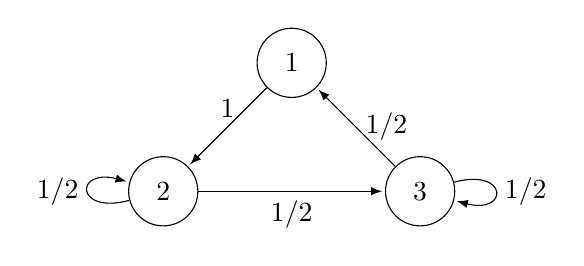
\begin{tikzpicture}

	\node[state] (1) {1};
	\node[state, below left=of 1] (2) {2};
	\node[state, below right=of 1] (3) {3};

	\draw[every loop, >=latex]
	(1) edge[above] node {$1$} (2)
	(2) edge[loop left] node {$1/2$} (2)
	(2) edge[below] node {$1/2$} (3)
	(3) edge[loop right] node {$1/2$} (3)
	(3) edge[right] node {$1/2$} (1);

	\end{tikzpicture}
	\end{center}

	This Markov chain has the transition matrix
	$$
	P = \begin{pmatrix}
		0 & 1 & 0 \\
		0 & 1/2 & 1/2 \\ 
		1/2 & 0 & 1/2
	\end{pmatrix},
	$$
	which has distinct eigenvalues $\{1, i/2, -i/2\}$.

	We can rewrite the complex eigenvalues using trigonometric functions as
	\begin{align*}
		\frac{i}{2} &= \cos \frac{\pi}{2} + i \sin \frac{\pi}{2}, \\ 
		-\frac{i}{2} &= \cos \frac{\pi}{2} - i \sin \frac{\pi}{2}.
	\end{align*}

	The general form for $p_{1,1}(n)$ is then given by
	$$
	p_{1n1}(n) = A + B \cdot \left(\frac{1}{2}\right)^n \cos \left(\frac{n \pi}{2}\right) + C \cdot \left(\frac{1}{2}\right)^n \sin\left(\frac{n \pi}{2}\right).
	$$
	The boundary conditions can be computed by hand as
	$p_{1,1}(0) = 1$, $p_{1,1}(1) = 0$ and $p_{1,1}(2) = 0$. This allows us to solve for $A$, $B$ and $C$ to get
	$$
	p_{1,1}(n) = \frac{1}{5} + \left(\frac{1}{2}\right)^n \left(\frac{4}{5}\cos\left(\frac{n \pi}{2}\right) - \frac{2}{5} \sin \left(\frac{n \pi}{2}\right)\right).
	$$
\end{example}

\section{Class Structure}

Test



\subsection{Communicating Classes}

\begin{definition}
$X$ is a Markov chain with transition matrix $P$ and values in $I$. For $x, y \in I$ we say that \vocab{$x$ leads to $y$} and write it $x \rightarrow y$ if
$$
\PP(X_m = y \text{ for some }n \geq 0) > 0. 
$$
We say that $x$ \vocab{communicates} with $y$ and write $x \longleftrightarrow y$ if both $x \rightarrow y$ and $y \rightarrow x$.  
\end{definition}

\begin{theorem}
	The following are equivalent: 
	\begin{enumerate}[label=(\roman*)]
		\item $x \rightarrow y$;
		\item There exists a sequence of states $x = x_0, x_1, \dots, x_k = y$ such that 
		$$P(x_0, x_1)P(x_1, x_2) \cdots P(x_{k - 1}, x_k) > 0;$$
		\item There exists $n \geq 0$ such that $p_{xy}(n) > 0$.
	\end{enumerate}
\end{theorem}
\begin{proof}
	Trivial.
\end{proof}

\begin{corollary}
	$\longleftrightarrow$ is an equivalence relation on $I$.
\end{corollary}
\begin{proof}
	Trivial.
\end{proof}

\begin{definition}[Communicating Classes]
	The equivalence classes induced by $\longleftrightarrow$ on $I$ are called \vocab{communicating classes}.
\end{definition}

A communicating class $C$ is \vocab{closed} if whenever $x \in C$ and $x \rightarrow y$ then $y \in C$.

A matrix $P$ is called \vocab{irreducible} if it has a single communicating class, that is, for all $x, y \in I$ we have $x \longleftrightarrow y$. 

A state $x$ is called \vocab{absorbing} if $\{x\}$ is a closed class. 

\subsection{Hitting Times}

\begin{definition}
	For $A \subseteq I$, we define $T_A$ to be the \vocab{hitting time} of $A$,
	$
	T_A: \Omega \rightarrow \{0, 1, 2, \dots \} \cup \{\infty\},
	$
	defined by $T_A(\omega) = \inf\{ n \geq 0: X_n(\omega) \in A\}$, where we take $\inf \emptyset = \infty$.

	The \vocab{hitting probability} of $A$ is $h^A: I \rightarrow [0, 1]$ such that $h_i^A = \PP_i(T_A < \infty)$.

	The \vocab{mean hitting time} of $A$ is $k^A: I \rightarrow \R$ with $k_i^A = \EE_i[T_A] = \sum_{n = 0}^{\infty} n \cdot \PP_i(T_a = n) + \infty \cdot \PP_i(T_a = \infty)$.
\end{definition}

\begin{example}
	Consider the Markov chain in the diagram below.
	\begin{center}
		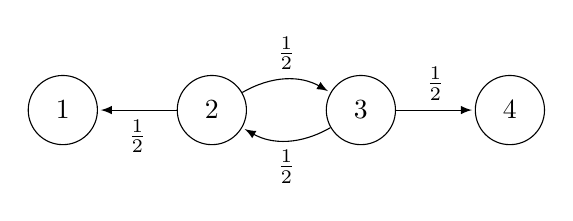
\begin{tikzpicture}
		
		\node[state] (1) {1};
		\node[state, right=of 1] (2) {2};
		\node[state, right=of 2] (3) {3};
		\node[state, right=of 3] (4) {4};
		
		\draw[every loop, >=latex]
		% (1) edge[loop above] node {1} (1)
		(2) edge[auto=left] node {$\frac{1}{2}$} (1)
		(2) edge[bend left, auto=left] node {$\frac{1}{2}$} (3)
		(3) edge[bend left, auto=left] node {$\frac{1}{2}$} (2)
		(3) edge[auto=left] node {$\frac{1}{2}$} (4);
		% (4) edge[loop above] node {1} (4);
		
		\end{tikzpicture}
		\end{center}

		We take $A = \{4\}$, and want to find $h_2^A = \PP_2(T_A < \infty)$. We have
		\begin{align*}
			h_2^A &= \frac{1}{2}h_3^A \\
			h_3^A &= \frac{1}{2} \cdot 1 + \frac{1}{2} h_2^A \\
		\implies h_2^A &= \frac{1}{3}.
		\end{align*}
		If instead we took $B = \{1, 4\}$ and wanted to find $k_2^B$, we would get
		\begin{align*}
			k_2^B &= 1 + \frac{1}{2}k_3^B \\
			k_3^B &= 1 + \frac{1}{2}k_2^B \\
	\implies k_2^B &= 2.
		\end{align*}
\end{example}

In the computations above, we really should check that this is a valid method (though it is quite intuitive).

\begin{theorem}
	Let $A \subseteq I$. The vector $(h_i^A)_{i \in A}$ is the minimal non-negative solution to
	\begin{align*}
		h_i^A = \begin{cases}
			1 &\mbox{if } i  \in A, \\
			\sum_{j} P(i, j) h_j^A &\mbox{if } i \not \in A,
		   \end{cases}
	\end{align*}
	where minimality means that if $(x_i)_{i \in A}$ is another solution to the linear system, then $x_i \geq h_i^A$ for all $i$.
\end{theorem}
\begin{proof}
	We first check that $h_i$ does indeed solve this system. 
\end{proof}

\end{document}

